\documentclass[10pt]{book}
\usepackage{latexsym}
\usepackage{natbib}
\usepackage{graphicx}
\usepackage{caption}
\usepackage{subcaption}
\usepackage{listings}
\usepackage{algorithm}
\usepackage{algpseudocode}
\usepackage{amsmath}
\usepackage{amssymb} 
\usepackage{amsthm}

\usepackage{color}
\usepackage{rotating}

\newtheorem{definition}{Definition}
\newtheorem{theorem}{Theorem}

\newcommand{\R}{\mathbb{R}}
\newcommand{\E}{\mathrm{E}}
\newcommand{\Cov}{\mathrm{Cov}}
\newcommand{\Var}{\mathrm{Var}}

% graphs in subdirectories
\graphicspath{{rldm15/}{RLLiterature/}}

\title{Parameterized Modular Inverse Reinforcement Learning}
\author{Shun Zhang}
\date{}

\begin{document}
\maketitle

\chapter{Introduction}

\chapter{Literature Review}
Markov Decision Process
MDP:
\begin{itemize}
\item State: $S$.
\item Action: $A$.
\item Transition: $P: S \times A \times S \rightarrow \mathcal{R}$.
\item Reward: $R: S \times A \times S \rightarrow \mathcal{R}$.
\end{itemize}



Abstraction on MDP
\begin{itemize}
  \item Aggregate states: feature extraction. 
  \item Aggregate actions: {\bf option}. 
  \item Decompose transition: factored MDP. 
  \item Decompose value (abstract MDP): {\bf HAM, hierarchical RL, modular RL}.
\end{itemize}



MDP with Option
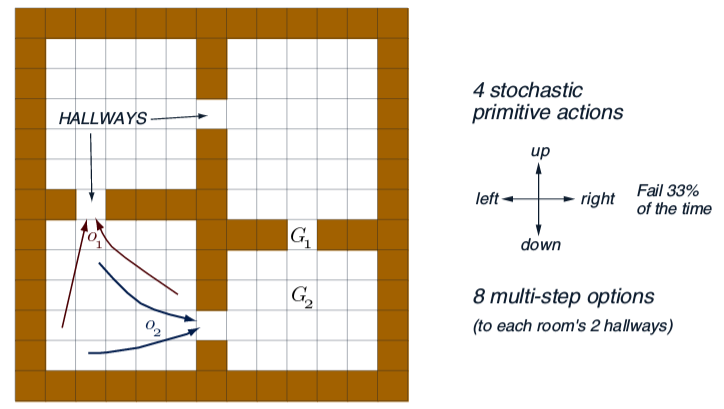
\includegraphics[width=0.8\columnwidth]{option.png}
\begin{itemize}
  \item Option: (start state, policy, termination condition).
\end{itemize}



\begin{itemize}
  \item State: $S$.
  \item Action: $A, {\color{red}O}$.
  \item Transition: $P: S \times {\color{red}\{A, O\}} \times S \rightarrow \mathcal{R}$.
  \item Reward: $R: S \times {\color{red}\{A, O\}} \times S \rightarrow \mathcal{R}$.
\end{itemize}



Hierarchies of Abstract Machines (HAM)
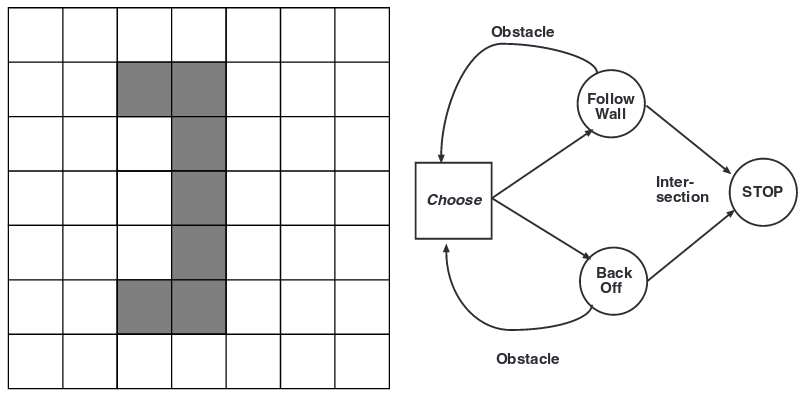
\includegraphics[width=0.8\columnwidth]{ham.png}
\begin{itemize}
  \item State machine of MDPs.
\end{itemize}



Hierarchical RL
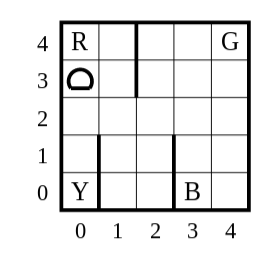
\includegraphics[width=0.4\columnwidth]{taxi.png}

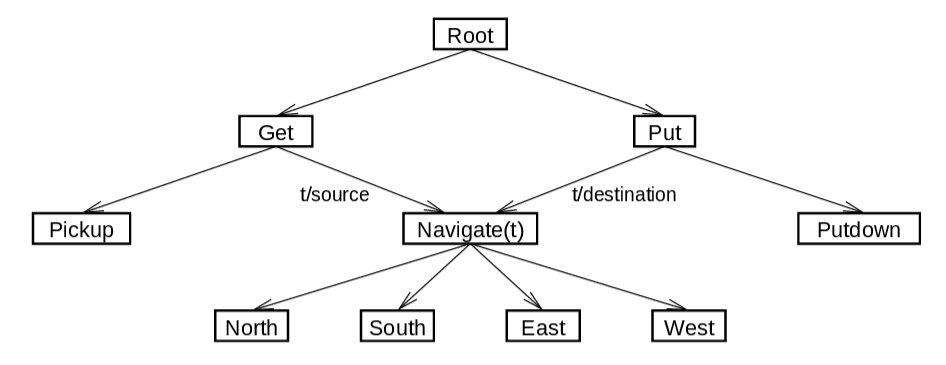
\includegraphics[width=0.8\columnwidth]{maxq.png}



Hierarchical RL
MDP:
\begin{itemize}
  \item State: {\color{red}$\mathcal{S}$}.
  \item Action: {\color{red}$\mathcal{A}$}.
  \item Transition: {\color{red}$\mathcal{T}$}.
  \item Reward: {\color{red}$\mathcal{R}$}.
\end{itemize}



Modular RL
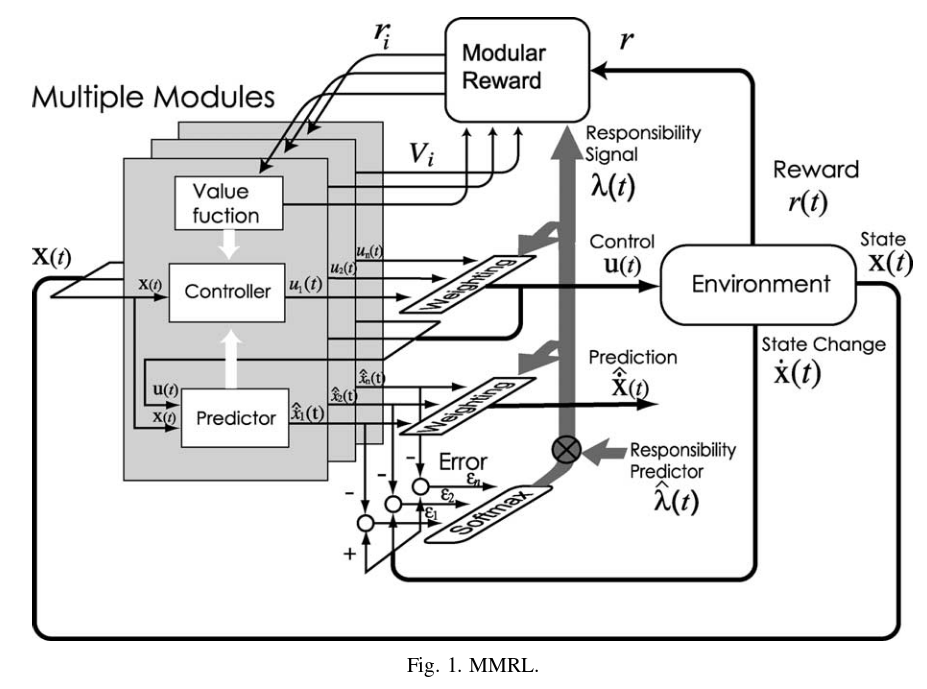
\includegraphics[width=0.8\columnwidth]{mrl.png}



MDP:
\begin{itemize}
  \item State: {\color{red}$S_1 \times S_2 \cdots \times S_M $}.
  \item Action: $A$.
  \item Transition: {\color{red}$P_1 \times P_2 \cdots \times P_M $}.
  \item Reward: {\color{red}$R_1 \times R_2 \cdots \times R_M $}.
\end{itemize}



Topics for Future Work
\begin{itemize}
  \item Credit assignment.
  \item Learning task hierarchies.
  \item Dynamic abstraction. 
  \item Integrating Deep Learning. 
\end{itemize}


\chapter{Parameterized Modular Inverse Reinforcement Learning}
\input{rldm15/3-irl}

\chapter{Application: Human Behavior Modeling}
\input{rldm15/2-domain}
\input{rldm15/4-experiments}
\input{rldm15/5-conclusion}

\chapter{Application: Influencing Agents in a Flock}
\begin{section}{Introduction}
Weighted sum of actions \cite{genter2015determining}.
\end{section}


\chapter{Conclusion}

\bibliographystyle{plain}
\bibliography{main,rldm15/paper,RLLiterature/report}

\end{document}
